\documentclass[12pt,titlepage]{article}
\usepackage[margin=1.25in]{geometry}
\usepackage{fancyhdr,tabularx,graphicx,tikz,longtable,tabu,amsmath}
\usetikzlibrary{svg.path,calc}
\tikzstyle{square} = [rectangle, draw, text centered, minimum height=2em, minimum width=5cm]
\tikzstyle{arrow} = [line width=0.5mm,->]

\usepackage{minted}
\definecolor{bg}{rgb}{0.08,0.09,0.12}
\definecolor{lightBg}{rgb}{0.8,0.8,0.8}
\usemintedstyle{github-dark}

\pagestyle{fancy}
\setlength{\headheight}{15pt} % compensate fancyhdr style
\fancyhead{}
\fancyfoot{}
\fancyfoot[L]{\thepage}
\fancyfoot[R]{\textit{Basic Programming Practicum - Jobsheet 3 Assignment}}
\renewcommand{\footrulewidth}{0.4pt}% default is 0pt, overline for footer

\newcommand{\details}[2]{
#1 & #2  \\
}

\begin{document}
\begin{titlepage}
    \centering
    \vfill
    {\bfseries\LARGE
        Basic Programming Practicum\\
        \vskip0.25cm
        Jobsheet 3 Assignment
    }
    \vfill
    
\includegraphics[width=6cm]{images/polinema-logo.png}
    \vfill
    {\textbf{Name}\\
        Dicha Zelianivan Arkana\\
        \vskip0.5cm
        \textbf{NIM}\\
        2241720002\\
        \vskip0.5cm
        \textbf{Class}\\
        1i\\
        \vskip0.5cm
        \textbf{Department}\\
        Information Technology\\
        \vskip0.5cm
        \textbf{Study Program}\\
        D-IV Informatics Engineering}
\end{titlepage}

\section{Assignment}
\begin{enumerate}
    \item {
        Pay attention to the following table.
        \begin{longtabu} to \textwidth {|l|l|l|l|}
            \hline \multicolumn{1}{|c|}{\textbf{Variable Name}} & \multicolumn{1}{c|}{\textbf{Data Type}} & \multicolumn{1}{c|}{\textbf{Initial Value}} & \multicolumn{1}{c|}{\textbf{Detail}} \\ \hline 
            \endfirsthead

            campus & Sentence & Polinema & -\\
            grade & Round Number & 1 & -\\
            class & Character & i & initial value = your class \\
            integer & Integers & 10 & -\\
            number & Floating point & 3.33333 & -\\
            character & Character & C & -\\

            \hline
        \end{longtabu}

        From the information provided on the table, create a program to display like this:

        \begin{minted}[autogobble, bgcolor=lightBg, fontsize=\footnotesize]{text}
            I am Polinema student, class 1i
            I'm learning to display values:
            Integer 10
            Floating point 3.33
            Character C
        \end{minted}

        \begin{figure}[h]
            \centering
            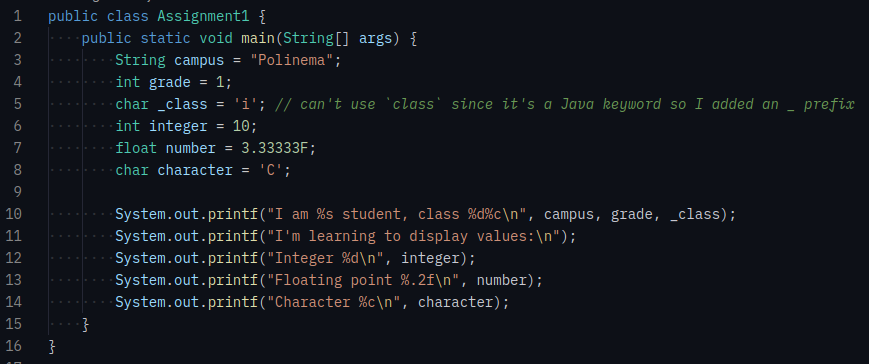
\includegraphics[width=0.9\textwidth]{./images/assignment1-code.png}
            \caption{The code for Assignment No. 1}
        \end{figure}
        \pagebreak
        \begin{figure}[h]
            \centering
            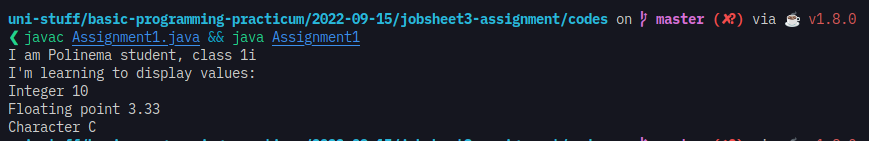
\includegraphics[width=0.9\textwidth]{./images/assignment1-output.png}
            \caption{The output for Assignment No. 1}
        \end{figure}
    }
    \item {
        Observe the following flowchart to convert the temperature

        \begin{figure}[h]
            \centering
            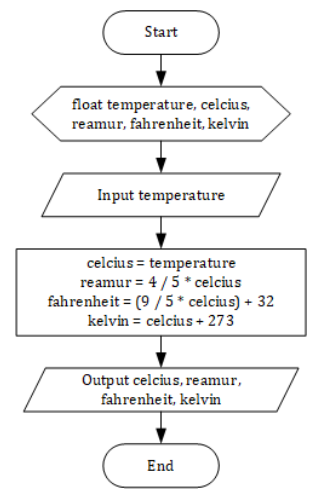
\includegraphics[width=0.5\textwidth]{./images/flowchart2.png}
        \end{figure}

        \pagebreak
        Implement the flowchart into the program using the Java programming language!

        \begin{figure}[h]
            \centering
            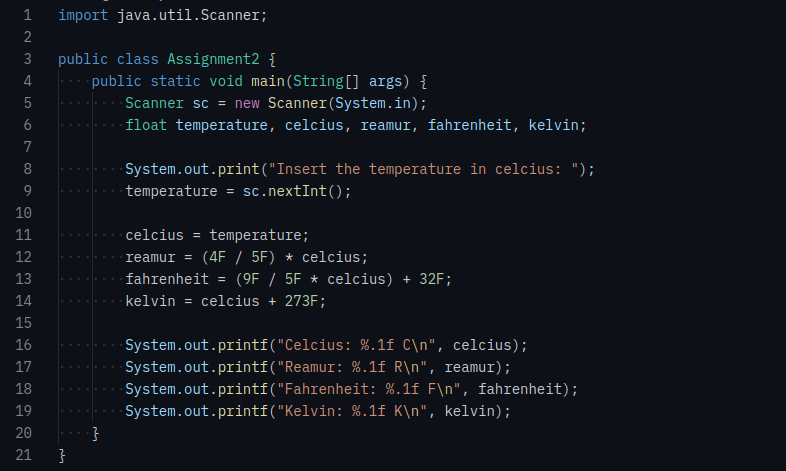
\includegraphics[width=0.9\textwidth]{./images/assignment2-code.png}
            \caption{The code for Assignment No. 2}
        \end{figure}
        \begin{figure}[h]
            \centering
            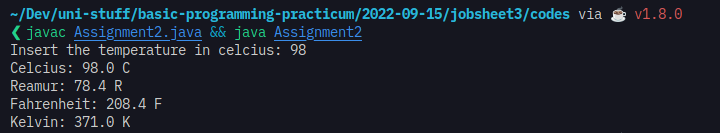
\includegraphics[width=0.9\textwidth]{./images/assignment2-output.png}
            \caption{The output for Assignment No. 2}
        \end{figure}
    }
\end{enumerate}

\end{document}

